% ============================================================
%  Informe Laboratorio 1 - Frecuencimetro digital sobre FPGA
%  Compilar con: pdflatex informe_lab1.tex  (dos veces)
% ============================================================
\documentclass[11pt,a4paper]{article}

\usepackage[utf8]{inputenc}
\usepackage[T1]{fontenc}
\usepackage[spanish,es-noquoting]{babel}
\usepackage{lmodern}
\usepackage[margin=2.2cm,top=1.9cm,bottom=1.9cm]{geometry}
\usepackage{graphicx}
\usepackage{booktabs}
\usepackage{amsmath}
\usepackage{tikz}
\usetikzlibrary{arrows.meta,positioning,calc}
\usepackage{caption}
\usepackage{enumitem}
\usepackage{xcolor}

\captionsetup{font=small,labelfont=bf}
\addto\captionsspanish{\renewcommand{\tablename}{Tabla}}
\setlist[itemize]{topsep=2pt,itemsep=1.5pt,parsep=0pt,leftmargin=1.2em}
\setlength{\parskip}{3pt}
\pagestyle{empty}

% --- estilos para los diagramas ---
\tikzset{
  blk/.style   = {draw, rounded corners=1.5pt, align=center, font=\footnotesize,
                  minimum height=8mm, inner xsep=4pt},
  blkg/.style  = {blk, fill=black!6},
  sig/.style   = {-{Latex[length=2mm]}, semithick},
  lbl/.style   = {font=\scriptsize, inner sep=1.5pt},
  st/.style    = {draw, circle, align=center, font=\scriptsize, minimum size=16mm},
}

% --- marca para los datos que faltan completar ---
\newcommand{\falta}[1]{\textcolor{red}{\textbf{[#1]}}}

\begin{document}

% ------------------------------------------------------------
\begin{center}
  {\large\bfseries Frecuencímetro digital sobre FPGA}\\[2pt]
  {\small Laboratorio 1 --- Sistemas Electrónicos de Instrumentación}\\[2pt]
  {\footnotesize Pedro Villar \quad\textbar\quad \today}
\end{center}
\vspace{-4pt}
\hrule
\vspace{6pt}

% ------------------------------------------------------------
\section*{1. Introducción}

Se implementó un frecuencímetro digital de cuatro dígitos en la placa \textbf{Boolean Board}
(FPGA Xilinx Spartan-7).

Usamos el \emph{método de medición directa}: se abre una ventana de tiempo conocida y se
cuentan los flancos de subida de la señal de entrada que caen dentro de esa ventana. 
\[
f_x=\frac{N_{\text{pulsos}}}{T_{\text{ventana}}}\, ,
\qquad\text{con } T_{\text{ventana}}=1\ \text{s}\ \Rightarrow\ f_x = N_{\text{pulsos}}\ \text{[Hz]}.
\]
Es decir, con una ventana de exactamente un segundo la cuenta acumulada \emph{es} la frecuencia en
hertz. El resultado se muestra en el display de la placa, con un rango de $0$ a $9999$~Hz.

% ------------------------------------------------------------
\section*{2. Arquitectura del diseño}

El sistema se dividió en módulos independientes, todos instanciados dentro del módulo \newline
\texttt{Frequency\_meter.sv}, que hace de \emph{top-level}. La Figura~\ref{fig:bloques} muestra cómo
quedan conectados.

\begin{figure}[h]
\centering
\begin{tikzpicture}[x=1cm,y=1cm,scale=0.88,every node/.style={transform shape}]

% ---------- fila de control ----------
\node[blk] (base) at (1.0,3.0) {Base de Tiempo\\ \texttt{BaseTime1ms}};
\node[blk] (fsm)  at (5.5,3.0) {Unidad de Control\\ (FSM, 3 estados)};
\node[lbl] (clk)  at (-1.7,3.0) {\texttt{clk} 100\,MHz};
\draw[sig] (clk) -- (base);
\draw[sig] (base) -- node[above,lbl]{\texttt{tick\_1ms}} (fsm);

% ---------- fila de datos ----------
\node[blk]  (sync) at (0,0)    {Sincronizador 2\,FF\\ + detector de flanco};
\node[draw,circle,inner sep=0.5pt,font=\scriptsize] (and) at (2.8,0) {AND};
\node[blkg] (bcd)  at (5.5,0)  {Banco de 4\\ contadores BCD};
\node[blkg] (lat)  at (9.0,0)  {Registro\\ Latch 16 bits};
\node[blk]  (disp) at (11.6,0) {Multiplexor\\ 7 segmentos};

\node[lbl,align=center] (fin) at (-2.9,0)  {señal incógnita\\ (\texttt{servo0})};
\node[lbl,align=center] (out) at (13.7,0)  {\texttt{D0\_SEG}\\ \texttt{D0\_AN}};
\draw[sig] (fin)  -- (sync);
\draw[sig] (sync) -- node[above,lbl]{pulso} (and);
\draw[sig] (and)  -- node[above,lbl]{\texttt{enable}} (bcd);
\draw[sig] (bcd)  -- node[above,lbl]{$4{\times}4$ bits} (lat);
\draw[sig] (lat)  -- (disp);
\draw[sig] (disp) -- (out);

% ---------- señales de control ----------
\draw[sig] (5.0,2.55) -- (5.0,2.05) -- (2.8,2.05) -- (and.north);
\node[lbl,above] at (4.0,2.05) {\texttt{cnt\_en}};

\draw[sig] (5.5,2.55) -- (bcd.north);
\node[lbl,right] at (5.56,1.80) {\texttt{cnt\_rst}};

\draw[sig] (6.0,2.55) -- (6.0,1.15) -- (9.0,1.15) -- (lat.north);
\node[lbl,above] at (7.5,1.15) {\texttt{latch\_en}};

\end{tikzpicture}
\caption{Diagrama de bloques del frecuencímetro. En gris, los bloques escritos;
el multiplexor de 7 segmentos nos lo dió el profesor.}
\label{fig:bloques}
\end{figure}

\subsection*{Decisiones de diseño}

\begin{itemize}
  \item \textbf{Base de tiempo en dos etapas.} En lugar de un único contador de 0 a 99.999.999
  (27 bits), se reutilizó el módulo \texttt{BaseTime1ms} provisto, que divide los 100~MHz y emite un
  pulso cada milisegundo, y se cuentan 1000 de esos pulsos dentro de la propia FSM. Quedan dos
  contadores chicos (17 y 10 bits) en vez de uno grande, y la ventana queda expresada en
  milisegundos.

  \item \textbf{Un solo dominio de reloj.} Todo el diseño es síncrono al reloj de 100~MHz. La señal
  incógnita \emph{no} se usa como reloj: se la muestrea como un dato más. Esto evita generar relojes
  derivados.

  \item \textbf{Sincronizador y detector de flanco.} La señal de entrada es asíncrona respecto del
  reloj, así que pasa primero por dos flip-flops en cascada y después por un tercero que guarda el valor anterior. Con
  \texttt{freq\_sync\_1 \& \textasciitilde freq\_prev} se obtiene un pulso de un único ciclo por
  cada flanco de subida, lo que garantiza que cada flanco incremente el contador exactamente una
  vez, sin importar el ancho del pulso de entrada.

  \item \textbf{La ventana es una compuerta AND.} El pulso de flanco se combina con \texttt{cnt\_en}
  de la FSM (\texttt{count\_pulse = freq\_edge \& cnt\_en}). Cuando la FSM cierra la ventana, el
  contador simplemente deja de recibir pulsos.

  \item \textbf{Contadores BCD en cascada en lugar de binario.} Cada dígito cuenta de 0 a 9 y genera
  un \texttt{carry\_out} de un ciclo que habilita al dígito siguiente. Así el resultado ya sale
  separado en dígitos decimales de 4 bits y se conecta directo al decodificador, sin necesidad de
  hacer divisiones sucesivas por 10 en hardware.

  \item \textbf{Registro latch para estabilizar la lectura.} Sin él, el display mostraría el conteo
  creciendo durante todo el segundo. El banco de flip-flops D captura el valor solo cuando la FSM
  activa \texttt{latch\_en}, de modo que en pantalla siempre se ve la última medición completa y el
  número se actualiza una vez por segundo.
\end{itemize}

\subsection*{Unidad de control (FSM)}

La unidad de control es una máquina de estados con un contador interno
\texttt{ms\_count} que acumula los \texttt{tick\_1ms} mientras dura la medición.

\begin{figure}[h]
\centering
\begin{minipage}[c]{0.60\textwidth}
\centering
\begin{tikzpicture}[x=1cm,y=1cm,scale=0.85,every node/.style={transform shape}]
  \node[st] (med) at (0,0)   {S\_MEDICION\\ {\tiny\texttt{cnt\_en=1}}};
  \node[st] (cap) at (5.2,0) {S\_CAPTURA\\ {\tiny\texttt{latch\_en=1}}};
  \node[st] (rei) at (2.6,-2.8) {S\_REINICIO\\ {\tiny\texttt{cnt\_rst=1}}\\ {\tiny\texttt{reset\_ms=1}}};

  \draw[sig] (med) -- node[above,lbl,align=center]
        {\texttt{tick\_1ms} \&\\ \texttt{ms\_count==999}} (cap);
  \draw[sig] (cap) -- node[right,lbl,pos=0.4]{1 ciclo} (rei);
  \draw[sig] (rei) -- node[left,lbl,pos=0.6]{1 ciclo} (med);

  \draw[sig] (med) to[out=115,in=65,looseness=7]
        node[above,lbl]{resto del tiempo} (med);
  \node[lbl] (r) at (-2.1,0) {\texttt{rst}};
  \draw[sig] (r) -- (med);
\end{tikzpicture}
\end{minipage}%
\begin{minipage}[c]{0.38\textwidth}
\centering
\footnotesize
\begin{tabular}{@{}lccc@{}}
\toprule
Estado & \texttt{cnt\_en} & \texttt{latch\_en} & \texttt{cnt\_rst} \\
\midrule
S\_MEDICION & 1 & 0 & 0 \\
S\_CAPTURA  & 0 & 1 & 0 \\
S\_REINICIO & 0 & 0 & 1 \\
\bottomrule
\end{tabular}
\\[4pt]
{\scriptsize Salidas de la unidad de control.}
\end{minipage}
\caption{Diagrama de estados de \texttt{FSM\_Control}.}
\label{fig:fsm}
\end{figure}

El ciclo de trabajo es el siguiente. En \textbf{S\_MEDICION} los contadores están habilitados y la
FSM espera a que lleguen 1000 ticks de 1~ms. En \textbf{S\_CAPTURA}, que dura un único ciclo de
reloj, se levanta \texttt{latch\_en} y el registro guarda el valor alcanzado. En
\textbf{S\_REINICIO}, también de un ciclo, se borran los contadores BCD y el contador de
milisegundos, y la máquina vuelve a medir. La lógica de próximo estado y de salidas está escrita en
un bloque \texttt{always\_comb} con valores por defecto asignados al principio, para que la síntesis
no infiera latches no deseados.


% ------------------------------------------------------------
\section*{3. Resultados y síntesis}

El diseño se sintetizó, se implementó y se cargó en la Boolean Board. Para la prueba se inyectó por
el pin \texttt{servo0} una señal desde un generador de funciones GW~Instek AFG-2005, de
$1{,}700$~V$_{pp}$ con un offset de $0{,}90$~V, y se comparó en paralelo la frecuencia ajustada en
el generador con lo que mostraban los displays de la placa.

\begin{table}[h]
\centering
\footnotesize
\caption{Frecuencia de prueba inyectada y lectura obtenida en los displays.}
\begin{tabular}{@{}llp{7.4cm}@{}}
\toprule
Frecuencia inyectada (generador) & Lectura en displays & Observación \\
\midrule
$7{,}894$~kHz & 7894~Hz & El dígito de los millares no aparece en la foto. Justo la camara no logro agarrar bien la foto, pero en la placa la lectura
se veía completa. \\
\bottomrule
\end{tabular}
\end{table}
\newpage
% Los dos recortes salen de la misma foto del banco de trabajo (foto_medicion.jpg,
% que quedó en esta carpeta). Si preferís mostrar la foto entera en vez de los dos
% detalles, reemplazá todo el bloque de abajo por:
%     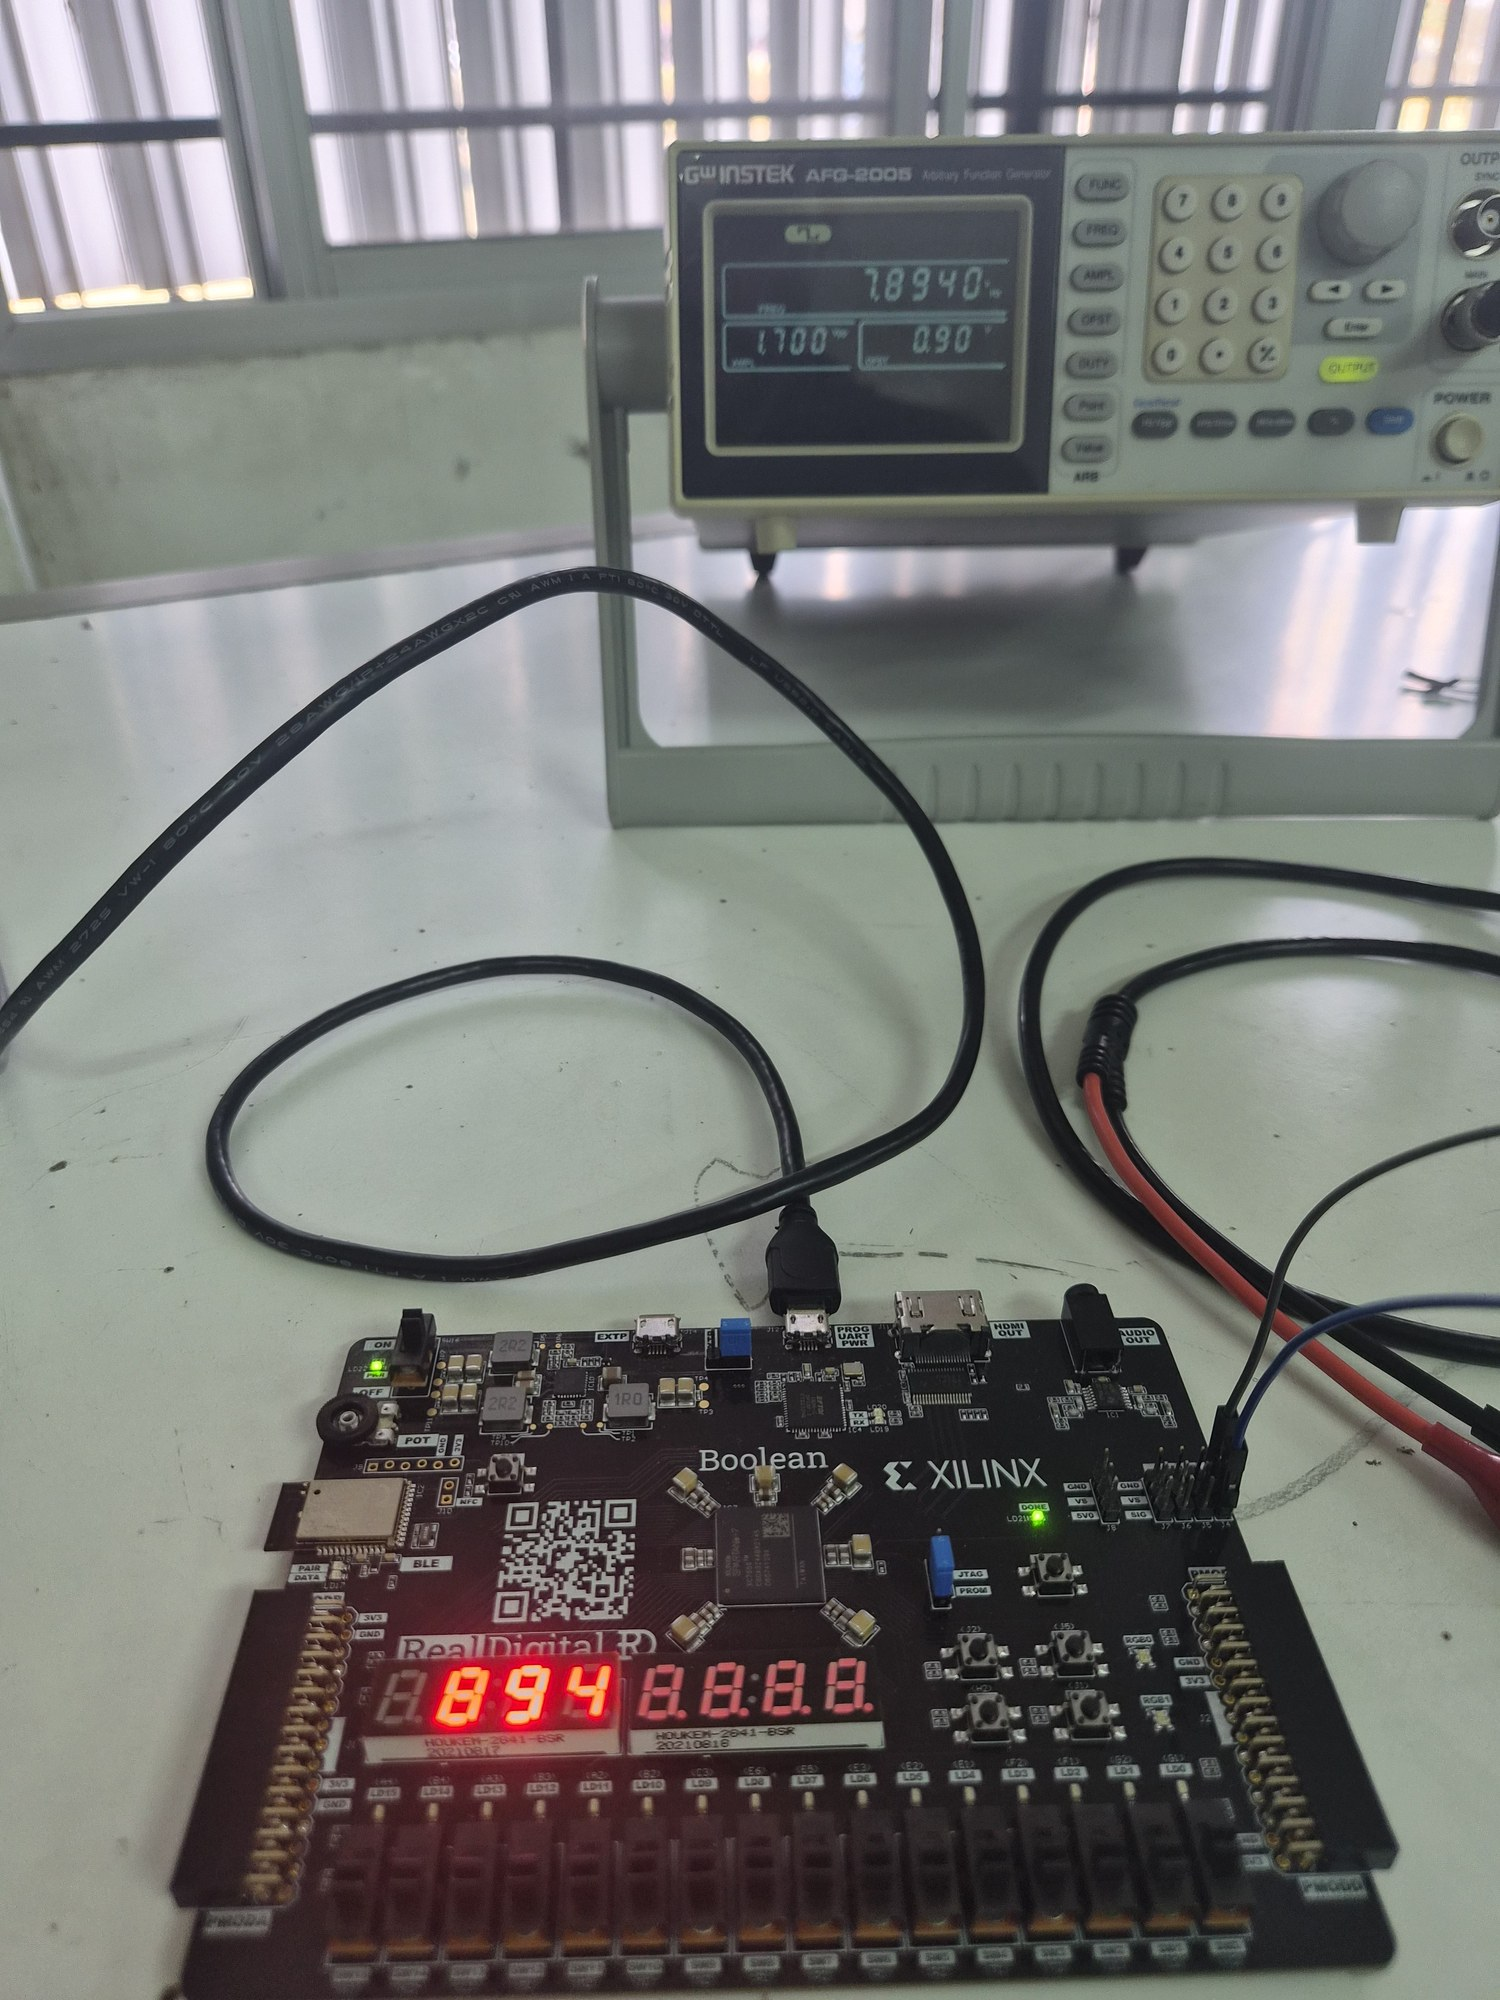
\includegraphics[width=0.40\textwidth]{foto_medicion.jpg}
\begin{figure}[h]
\centering
\begin{minipage}[t]{0.48\textwidth}
  \centering
  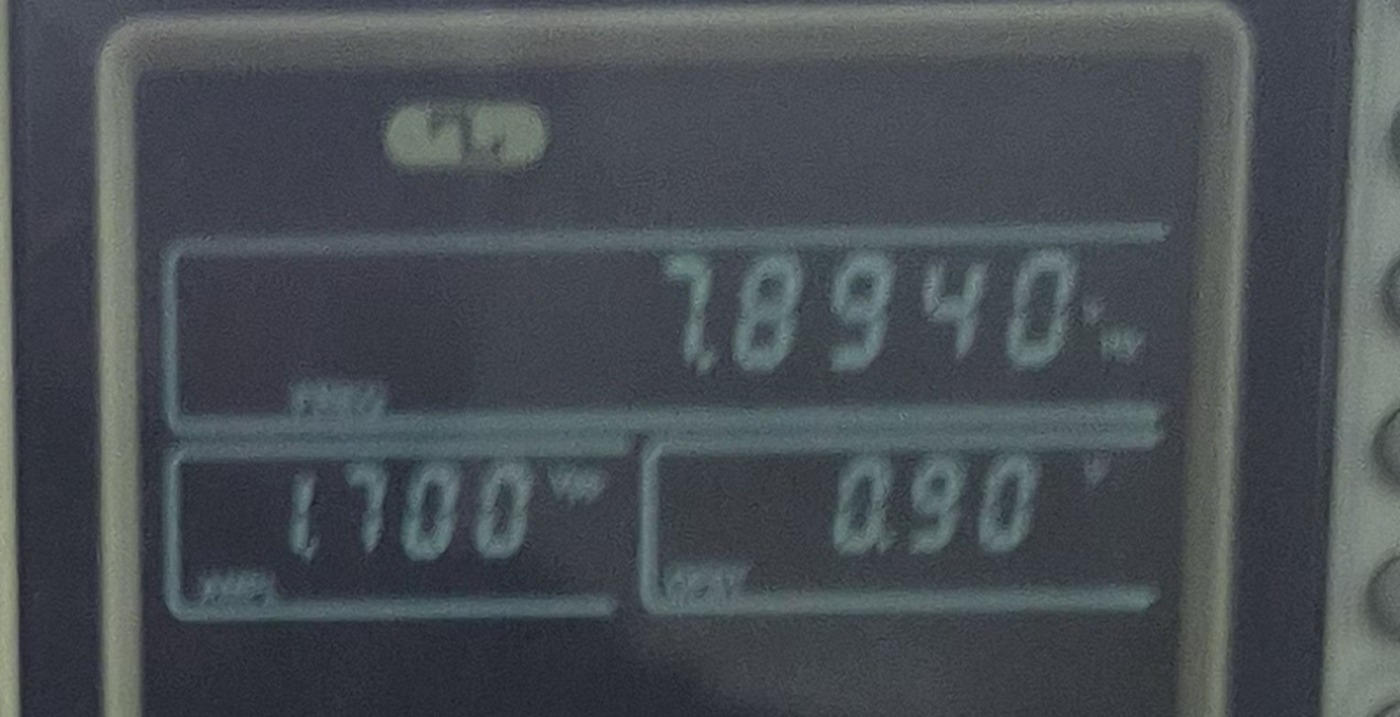
\includegraphics[width=\linewidth]{foto_generador.jpg}\\[2pt]
  {\scriptsize (a) Generador: FREQ $=7{,}8940$~kHz}
\end{minipage}\hfill
\begin{minipage}[t]{0.48\textwidth}
  \centering
  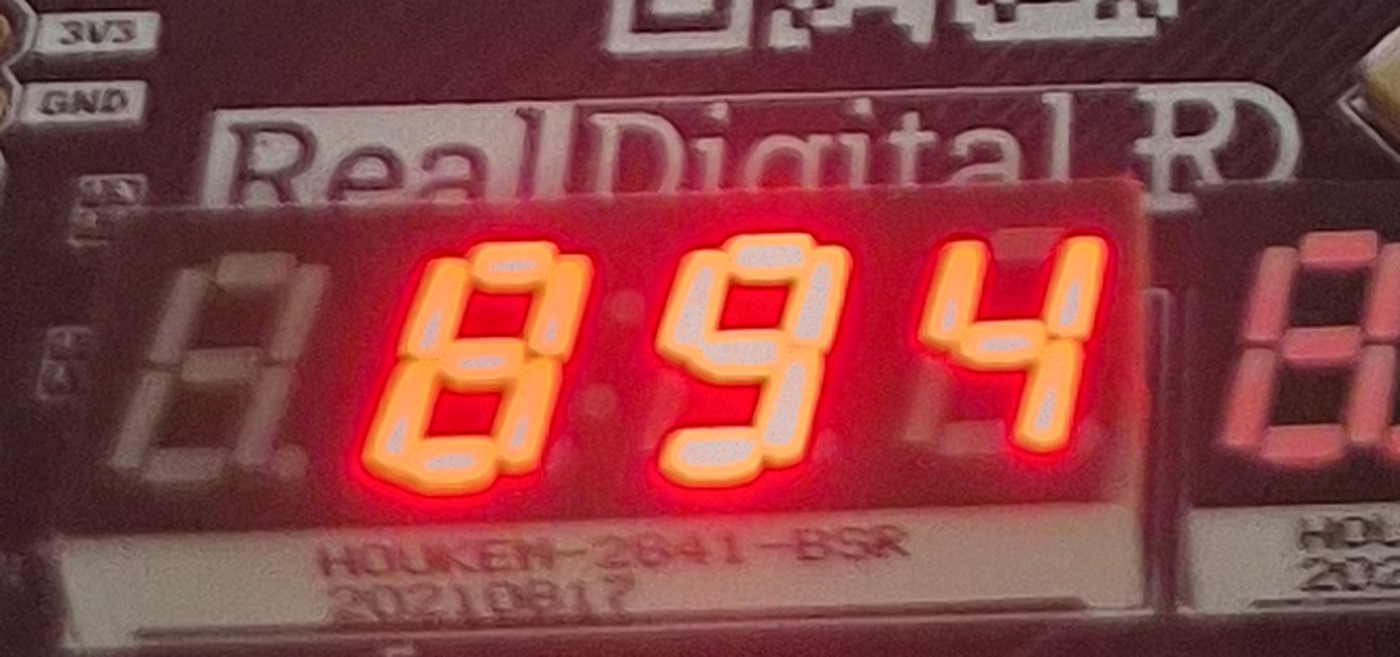
\includegraphics[width=\linewidth]{foto_displays.jpg}\\[2pt]
  {\scriptsize (b) Display de la Boolean Board}
\end{minipage}
\caption{Medición sobre la placa. A la izquierda, la frecuencia ajustada en el generador de
funciones; a la derecha, el valor contado por el frecuencímetro en el display de siete segmentos.}
\label{fig:medicion}
\end{figure}

\paragraph{Costo espacial del diseño.}
La Tabla~\ref{tab:util} resume los recursos que reportó Vivado en el \emph{Utilization Report}
después de la implementación.

\begin{table}[h]
\centering
\footnotesize
\caption{Recursos utilizados. Vivado 2024.2, post-implementación, dispositivo
\texttt{xc7s50csga324-1}.}
\label{tab:util}
\begin{tabular}{@{}lrrr@{}}
\toprule
Recurso & Usados & Disponibles & Utilización \\
\midrule
LUTs (Slice LUTs)            &  51 & 32.600 & 0,16\,\% \\
Flip-Flops (Slice Registers) & 105 & 65.200 & 0,16\,\% \\
Bonded IOB (pines)           &  15 &    210 & 7,14\,\% \\
\bottomrule
\end{tabular}
\end{table}


% ------------------------------------------------------------
\section*{4. Conclusión}

Lo que más me costó al principio fue asimilar que acá no estoy programando, sino describiendo. La
secuencialidad del código, que en software es la base fundamental de todo lo que uno hace, deja de
existir: no hay una línea que se ejecute después de la otra, sino bloques que quedan instanciados y
funcionando en paralelo. Eso complica además la forma de depurar, porque las cosas no se disparan
como en un programa y uno pierde la referencia de por dónde va la ejecución. De todas formas, me
parece que el aprendizaje más importante no pasa por ahí, sino por ver la diferencia entre ejecutar
una tarea sobre un micro ya armado y ejecutarla directamente sobre compuertas. Corriendo sobre la
FPGA obviamente se gana velocidad, pero se complica bastante más, porque no estamos trabajando
sobre un sistema operativo que nos resuelva todo lo que hay por debajo. Ahí es donde me parece que
está lo más valioso de este trabajo: entender el \emph{trade-off} entre resolver algo en hardware o
resolverlo en firmware.

\end{document}
